\documentclass[12pt,a4paper]{scrartcl}
\usepackage[brazil]{babel}
\usepackage[T1]{fontenc}
\usepackage[utf8]{inputenc}
\usepackage[onehalfspacing]{setspace}
\usepackage{graphicx}
\usepackage{hyperref}

\usepackage{amssymb,amsfonts,amsmath,amsthm}
\usepackage{mathtools}
\usepackage{latexsym}
\usepackage[brazilian]{cleveref}

\usepackage{float}
\usepackage[table]{xcolor}
\usepackage{indentfirst}
\usepackage{dsfont}
\usepackage{caption}
\usepackage{subcaption}

\DeclareMathOperator{\proj}{proj}
\DeclareMathOperator*{\argmax}{arg\, max}
\DeclareMathOperator*{\argmin}{arg\, min}
\DeclareMathOperator{\diag}{diag}
\DeclareMathOperator{\ones}{ones}
\DeclareMathOperator{\dist}{dist}

\def\Xset{\mathcal{X}}
\def\Yset{\mathcal{Y}}
\def\Hset{\mathcal{H}}
\def\RR{\mathds{R}}
\def\xbar{\bar{x}}
\def\wbar{\bar{w}}
\def\bbar{\bar{b}}


\newtheorem{teorema}{Teorema}%ambientes em itálico
\newtheorem{prop}{Proposição}
\newtheorem{teo}{Teorema}
\newtheorem{lema}{Lema}

\theoremstyle{definition}%ambientes normais
\newtheorem{exem}{Exemplo}[subsection]
\newtheorem{defi}{Definição}
\newtheorem{obs}{Observação}	

\usepackage{csquotes}
\usepackage[
backend=biber,
style=numeric-comp, noerroretextools=true, sorting=nty,
]{biblatex}
\addbibresource{referencias.bib}

 \let\etoolboxforlistloop\forlistloop % save the good meaning of \forlistloop
 \usepackage{autonum}
 \let\forlistloop\etoolboxforlistloop % restore the good meaning of \forlistloop
 
 
\begin{document}

\title{Métodos de Otimização e Máquinas de Vetores Suporte} 
\author{ \normalfont Paula Cristina Rohr Ertel\thanks{Acadêmica do curso de Licenciatura em Matemática/UFSC-Blumenau} \\ \small Orientador: Luiz Rafael dos Santos \\ \small Universidade Federal de Santa Catarina - Campus Blumenau}
\date{\small 18 de Novembro de 2019}
\subtitle{Qualificação de Trabalho de Conclusão de Curso}
\maketitle

\section{Introdução às Máquinas de Vetores Suporte}

A Aprendizagem de Máquina (do inglês \textit{Machine Learning}) é o estudo do uso de técnicas computacionais para automaticamente detectar padrões em dados e usá-los para fazer predições e tomar decisões. De acordo com \textcite{Evelin2017}, existem dois tipos de Aprendizagem de Máquina, a aprendizagem supervisionada, em que a partir de um conjunto de dados de entrada e saída a máquina constrói um modelo que deduz a saída para novas entradas, e a não supervisionada, na qual a máquina cria sua própria solução. 

A aprendizagem supervisionada é composta por uma etapa denominada fase de treinamento, na qual é dado um conjunto de treinamento formado por vários dados de entrada e saída que funcionam como exemplos, a partir dos quais a máquina detecta padrões e cria um modelo para deduzir a saída de novos dados. Após essa fase novas entradas são testadas, denominadas conjunto de teste, no intuito de analisar se a máquina está gerando as saídas corretas. Algumas técnicas para aprendizagem de máquina supervisionada são as Máquinas de Vetores Suporte, Regressão Linear, Regressão Logística e Redes Neurais. Enquanto que a \textit{Singular Value Decomposition} (SVD), Clusterização e Análise de Componentes Principais \cite{Evelin2017} são exemplos de técnicas para a aprendizagem não supervisionada. 

As Máquinas de Vetores Suporte (SVM, do inglês \textit{Support Vector Machine}), conforme mencionado por \textcite{Evelin2017}, são indicadas nos casos em que ocorrem dados de dimensões elevadas e com altos níveis de ruídos, além de apresentar uma boa capacidade de generalização. Esta técnica pode ser aplicada tanto para problemas de regressão como de classificação. Segundo \textcite{Evelin2017}, essa técnica foi desenvolvida por Vladimir Vapnik, Bernhard Boser, Isabelle Guyon e Corrina Cortes, com base na Teoria de Aprendizagem Estatística. Algumas aplicações de SVM em problemas práticos são o reconhecimento facial, leitura de placas automotivas e detecção de spam.

Agora, vamos formular matematicamente o problema de classificação utilizando as Máquinas de Vetores Suporte. Para tanto, considere um conjunto de dados, pertencentes a duas classes distintas, conforme \Cref{fig1}.


\begin{figure}[!h] 
\centering
\begin{subfigure}[h]{0.3\textwidth}
\centering
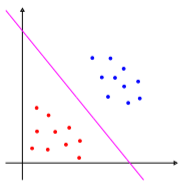
\includegraphics[width=\textwidth]{SVM_linear}
\caption{Linear. \label{fig1:a}}
\end{subfigure}
\begin{subfigure}[!h]{0.3\textwidth}
	\centering
	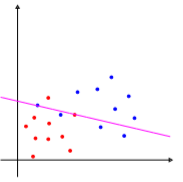
\includegraphics[width=\textwidth]{SVM_flexivel}
	\caption{Flexível. \label{fig1:b}}
\end{subfigure}
\begin{subfigure}[!h]{0.3\textwidth}
	\centering
	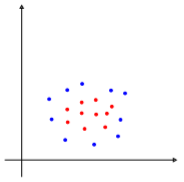
\includegraphics[width=\textwidth]{SVM_naolinear}
	\caption{Não Linear. \label{fig1:c}}
\end{subfigure}
\caption{Dados lineares, com margem flexível e não lineares. \label{fig1}\\ Fonte: \textcite{Evelin2017}}
\end{figure}

Observe que na \Cref{fig1:a} os dados podem ser classificados corretamente através de uma reta. Já na \Cref{fig1:b} é possível encontrar uma reta que separa alguns poucos dados, porém incorretamente. E na \Cref{fig1:c} não é possível classificar os dados como nos casos anteriores. Nestes exemplos temos representados os três casos de SVM: o linear com margem rígida, o linear com margem flexível e o não linear, respectivamente.

A modelagem do problema de classificação, utilizando a técnica de SVM, consiste em encontrar um hiperplano ótimo que melhor separe os dados de entrada $x^i$ em duas saídas $y_i$ através de uma função de decisão. Matematicamente, mostraremos que trata-se um problema de programação quadrática convexa com restrições lineares, que pode ser formulado como
\[
\begin{aligned}
\min_{w,b} & \quad f(w) \\
\text{s.a.} &  \quad g(w,b) \leq 0, \end{aligned}
\]
com $w\in \RR^n$ e $b\in \RR $, em que $f: \RR^n \rightarrow \RR$ é uma função quadrática e $g: \RR^{n+1} \rightarrow \RR^m$ é linear. Note também que $f$ e $g$ são continuamente diferenciáveis.



Para formular matematicamente o problema de classificação, considere os conjuntos de entrada $\Xset =\{x^1, \ldots , x^m \} \subset \RR^n$ e de treinamento $\Yset=\{(x^1, y_1), \ldots , (x^m, y_m)\mid x^i \in \Xset \, e \, y_i \in \{-1,1\}\}$, com a partição 
\[ \label{conj1}
\Xset ^{+} =\{x^i \in \Xset\mid y_i=1\} \quad e \quad \Xset^{-}=\{x^i \in \Xset\mid y_i=-1\},
\]
dos conjuntos formados pelos atributos pertencentes às classes positiva e negativa, respectivamente.

\begin{defi} Considere um vetor não nulo $w\in \RR^n$ e um escalar $b\in \RR$. Um hiperplano com vetor normal $w$ e constante $b$ é um conjunto da forma $\Hset(w,b)=\{x\in \RR^n \mid w^{T}x+b=0\}$.
\end{defi}

O hiperplano $\Hset(w,b)$ divide o espaço $\RR^n$ em dois semiespaços, dados por
\[ \label{conj2}
\mathcal{S}^{+}=\{x\in \RR^n \mid w^{T}x+b\geq 0\} \quad e \quad \mathcal{S}^{-}=\{x\in \RR^n \mid w^{T}x+b\leq 0\}.
\]


Considere dois conjuntos de dados de treinamento representados no $\RR^2$ como na \Cref{fig2:a}, em que os pontos em azul representam a classe positiva, e os pontos em vermelho a classe negativa. Perceba na \Cref{fig2:b} que todos os hiperplanos representados separam corretamente os dados, porém nosso objetivo será encontrar o hiperplano que melhor separa esses dados, o qual está representado na \Cref{fig3:a} pela cor violeta. Logo, desejamos encontrar o hiperplano que possibilita a maior faixa que não contém nenhum dado, pois caso a faixa seja muito estreita pequenas perturbações no hiperplano ou no conjunto de dados podem resultar uma classificação incorreta. 
\begin{figure}[htbp] 
	\centering
	\begin{subfigure}[h]{0.4\textwidth}
		\centering
		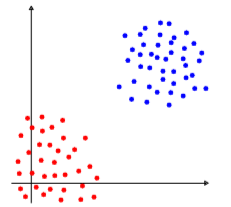
\includegraphics[width=\textwidth]{dados_treinamento}
		\caption{Dados de treinamento. \label{fig2:a}}
	\end{subfigure}
	\begin{subfigure}[h]{0.38\textwidth}
		\centering
		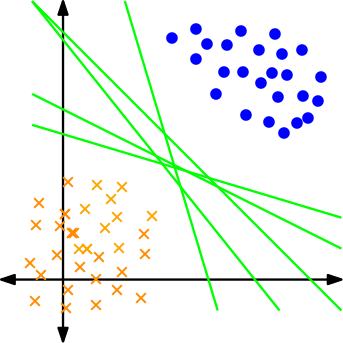
\includegraphics[width=\textwidth]{hiperplanos_separadores}
		\caption{Hiperplanos separadores. \label{fig2:b}}
	\end{subfigure}
\caption{Conjunto de Dados e Hiperplanos. \label{fig2}
	\\ Fonte: \textcite{Evelin2017}}
\end{figure}
\begin{figure}[hbtp] 
	\centering
	\begin{subfigure}[h]{0.38\textwidth}
		\centering
		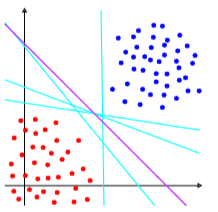
\includegraphics[width=\textwidth]{hiperplano_otimo}
		\caption{Hiperplano ótimo. \label{fig3:a}}
	\end{subfigure}
	\begin{subfigure}[h]{0.38\textwidth}
		\centering
		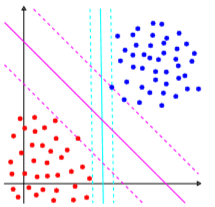
\includegraphics[width=\textwidth]{maxima_margem}
		\caption{Máxima margem. \label{fig3:b}}	
	\end{subfigure}
\caption{Hiperplano Ótimo. \label{fig3}
\\ Fonte: \textcite{Evelin2017}}
\end{figure}


\begin{defi} \label{def1} Os conjuntos $\Xset^{+}, \Xset^{-} \subset \RR^n$ são ditos linearmente separáveis quando existem $w\in \RR^n$ e $b\in \RR$  tais que $w^{T}x+b>0$ para todo $x\in \Xset^{+}$ e $w^{T}x+b<0$ para todo $x\in \Xset^{-}$. O hiperplano $\Hset(w,b)$ é chamado hiperplano separador dos conjuntos $\Xset^{+}$ e $\Xset^{-}$.
\end{defi}


\begin{lema} \label{lema1} Suponha que os conjuntos $\Xset^{+}, \Xset^{-} \subset \RR^n$ são finitos e linearmente separáveis, com hiperplano separador $\Hset(w,b)$. Então, existem $\overline{w}\in \RR^n$ e $\overline{b}\in \RR$ tais que $\Hset(w,b)$ pode ser descrito por
\[
\wbar^{T}x+\bbar =0,
\]
satisfazendo
\begin{align}
\wbar^{T}x+\bbar &\geq 1, \text{ para todo } x\in \Xset^{+}, \label{eq1} \\
\wbar^{T}x+\bbar &\leq -1, \text{ para todo } x\in \Xset^{-}. \label{eq2}
\end{align}
\end{lema} 

\begin{proof}
Pela  \Cref{def1}, temos que existem $w\in \RR^n$ e $b\in \RR$ tais que
\begin{align}
w^{T}x+b &>0, \text{ para todo } x\in \Xset^{+}, \\
w^{T}x+b &<0, \text{ para todo } x\in \Xset^{-}.
\end{align}  

Como $\Xset^{+}\cup \Xset^{-}$ é um conjunto finito, podemos definir
\[ \gamma \coloneqq \min_{x\in \Xset^{+}\cup \Xset^{-}} \vert w^{T}x+b\vert  >0. \]

Portanto, para todo $x\in \Xset^{+}\cup \Xset^{-}$, $\gamma \leq \vert w^{T}x+b\vert$ e consequentemente, $\dfrac{\vert w^{T}x+b\vert }{\gamma} \geq 1$. Assim, para $x\in \Xset^{+}$ temos
\[ \dfrac{w^{T}x+b}{\gamma} = \dfrac{\vert w^{T}x+b\vert }{\gamma} \geq 1, \]
e para $x\in \Xset^{-}$, temos
\[- \dfrac{w^{T}x+b}{\gamma} = \dfrac{\vert w^{T}x+b\vert }{\gamma} \geq 1. \]

Logo, definindo $\wbar:=\dfrac{w}{\gamma}$ e $\bbar :=\dfrac{b}{\gamma}$, obtemos as desigualdades \eqref{eq1} e \eqref{eq2}. 

\end{proof}


A partir do \Cref{lema1} temos que $\Hset^{+}:=\{x\in \RR^n \mid w^{T}x+b= 1\}$ e $\Hset^{-}:=\{x\in \RR^n \mid w^{T}x+b= -1\}$ são os hiperplanos que definem a faixa que separa os conjuntos $\Xset^{+}$ e $\Xset^{-}$.

\begin{prop} \label{prop1} A projeção ortogonal de um vetor $\xbar\in \RR^n$ sobre um hiperplano afim $\Hset(w,b)$, é dada por
\[ \proj_{\Hset}(\xbar)= \xbar - \dfrac{w^{T}\xbar+b}{w^{T}w}w. \]
Além disso, a $\proj_{\Hset}(\xbar)$ satisfaz a menor distância.
\end{prop}

\begin{proof}
Sejam $w\in \RR^n$ o vetor normal ao hiperplano $\Hset(w,b)$, $\bar{z}\in \Hset(w,b)$ e $x^{*}$ a projeção ortogonal de $\xbar$ sobre $\Hset(w,b)$. Assim, temos que 
\[ \label{eq3} w^{T}(x^{*}-\bar{z})=0 \]
e
\[ \label{eq4} \xbar-x^{*}=\lambda w \Longrightarrow x^{*}=\xbar-\lambda w. \]

Substituindo \eqref{eq4} em \eqref{eq3}, obtemos
\begin{align}
0 &= w^{T}(\xbar-\lambda w-\overline{z}) \\
&= w^{T}\xbar-\lambda w^{T}w - w^{T}\bar{z}.
\end{align}

Resolvendo para $\lambda$ e como $w^{T}\bar{z} = -b$, temos
\[ \lambda =\dfrac{w^{T}\xbar-w^{T}\bar{z}}{w^{T}w} =\dfrac{w^{T}\xbar+b}{w^{T}w}. \]

Portanto, 
\[ x^{*}=\xbar-\dfrac{w^{T}\xbar+b}{w^{T}w}w . \]

Ademais, vamos provar que a $\proj_{\Hset}(\xbar)$ satisfaz a menor distância, isto é,
\[ \Vert\xbar-x^{*}\Vert_{2} \leq \Vert \xbar-x\Vert_{2}, \]
para todo $x\in \Hset(w,b)$.

De fato, tomando $u=\xbar-x^{*}$ e $v=x^{*}-x$ observe que 
\begin{align}
u^{T}v&= (\xbar-x^{*})^{T}(x^{*}-x) \\
&= (\xbar-\xbar+\lambda w)^{T}(x^{*}-x) \\
&= \lambda w^{T}(x^{*}-x) \\
&= \lambda (w^{T}x^{*}-w^{T}x) \\
&= \lambda (-b-(-b)) \\
&= 0.
\end{align}

Assim, temos
\[ \Vert u+v\Vert^{2}=\Vert u\Vert^{2} + 2u^{T}v + \Vert v\Vert^{2}=\Vert u\Vert^{2} + \Vert v\Vert^{2} , \]
ou seja,
\[ \Vert \xbar-x\Vert^{2}=\Vert \xbar-x^{*}\Vert^{2} + \Vert x^{*}-x\Vert^{2}. \]

\end{proof}


Utilizando a \Cref{prop1} podemos demonstrar o \Cref{lema2}, o qual estabelece a largura da faixa entre os hiperplanos separadores $\Hset^{+}$ e $\Hset^{-}$.

\begin{lema} \label{lema2} A distância entre os hiperplanos $\Hset^{+}$ e $\Hset^{-}$ é dada por $\dist(\Hset^{+}, \Hset^{-})=\dfrac{2}{\Vert w\Vert}$. 
\end{lema}
\begin{proof}
Considere um ponto arbitrário $\xbar\in \Hset^{+}$ e seja $x^{*}\in \Hset^{-}$ a projeção ortogonal de $\xbar$ sobre $\Hset^{-}$. Usando a \Cref{prop1}, temos
\[ \label{eq6} x^{*}= \proj_{\Hset^{-}}(\xbar)= \xbar - \dfrac{w^{T}\xbar+b+1}{\Vert w\Vert^{2}}w. \] 

Além disso, a distância entre dois conjuntos é definida por
\[ \dist(\Hset^{+}, \Hset^{-}):= \inf\{\Vert x^{+}-x^{-} \Vert : x^{+}\in \Hset^{+} \ \text{e} \ x^{-}\in \Hset^{-}\},
\]
e como a $\proj_{\Hset^{-}}(\xbar)$ satisfaz a menor distância entre $\xbar$ e $\Hset^{-}$, e $\Hset^{+}$ é paralelo a $\Hset^{-}$, temos que 
\[ \label{eq7} \dist(\Hset^{+},\Hset^{-})=\Vert \xbar-x^{*}\Vert. \]

Substituindo \eqref{eq6} em \eqref{eq7} obtemos
\begin{align} 
\dist(\Hset^{+},\Hset^{-}) &= \Vert \xbar-x^{*}\Vert \\
&= \left\Vert \xbar -\xbar +\dfrac{w^{T}\xbar+b+1}{\Vert w\Vert^{2}}w \right\Vert \\
&=  \dfrac{\vert w^{T}\xbar+b+1 \vert}{\Vert w\Vert^{2}} \Vert w\Vert \\
&= \dfrac{\vert w^{T}\xbar+b+1 \vert}{\Vert w\Vert},
\end{align}
e como $\xbar\in \Hset^{+}$,  $ w^{T}\xbar+b=1$ implica
\[  w^{T}\xbar =1-b, \]
concluindo que 
\begin{align} 
\dist(\Hset^{+},\Hset^{-})&= \dfrac{\vert 1-b+b+1 \vert}{\Vert w\Vert} \\
&= \dfrac{2}{\Vert w\Vert }. 
\end{align}
\end{proof}

%--------------------------------------------------------------------------------------------------------------------------

\subsection{Formulação Matemática do Problema de Classificação - Margem Rígida}

Encontrar o hiperplano que melhor separa os dados implica maximizar a largura da margem, isto é, maximizar $\dist(\Hset^{+} , \Hset^{-}) =\dfrac{2}{\Vert w\Vert }$. Isso equivale a minimizar seu inverso $\dfrac{1}{2}\Vert w\Vert $ ou ainda minimizar $\dfrac{1}{2}\Vert w\Vert^{2}$. De fato, seja $w^{*}=\argmax\dfrac{2}{\Vert w\Vert}$. Então, para todo $w\in \RR^n$,
\[ \dfrac{2}{\Vert w^{*}\Vert} \geq \dfrac{2}{\Vert w\Vert} \]
implica
\[ \label{eq8} \Vert w\Vert \geq \Vert w^{*}\Vert. \]
Logo, $w^{*}=\argmin\Vert w\Vert$. Além disso, como $\Vert \cdot \Vert$ é não negativa, elevando ao quadrado ambos os lados da desigualdade \eqref{eq8} temos que  $\Vert w\Vert^{2} \geq \Vert w^{*}\Vert^{2}$ implica
\[ \dfrac{1}{2}\Vert w\Vert^{2} \geq \dfrac{1}{2}\Vert w^{*}\Vert^{2}. \]

Portanto, 
\[ \argmax\dfrac{2}{\Vert w\Vert} = \argmin\dfrac{1}{2}\Vert w\Vert^2. \]

Ademais, como a faixa deve separar os dados das duas classes, as seguintes restrições devem ser satisfeitas
\begin{align}
w^{T}x+b &\geq 1 , \text{ para  todo } x\in \Xset^{+}, \\
w^{T}x+b &\leq -1 , \text{ para  todo } x\in \Xset^{-}.
\end{align}

Considerando que $\Xset^{+}=\{x^i \in \Xset\mid y_i=1\}$ e $\Xset^{-}=\{x^i \in \Xset \mid y_i=-1\}$, podemos reescrever as restrições acima de uma forma mais compacta 
\[ y_{i}(w^{T}x^{i}+b)\geq 1, \quad i=1, \ldots ,m. \]

Portanto, o problema de encontrar o hiperplano ótimo pode ser formulado da seguinte maneira
\[ \label{eq:problemageralSVM}
\begin{aligned}
\min_{w,b} & \quad \dfrac{1}{2} \Vert w\Vert^{2} \\
\text{s.a.} &  \quad y_i(w^{T}x^{i}+b) \geq 1, \quad i=1, \ldots , m, \end{aligned}
 \]
em que $w\in \RR^{n}$ e $b\in \RR$. 

O problema \eqref{eq:problemageralSVM} possui função objetivo 
\[ f(w,b)=\dfrac{1}{2}\Vert w\Vert^{2} \]
convexa, e restrições lineares
\[ g_i(w,b)=1-y_i(w^{T}x^{i}+b) \leq 0, \quad i=1, \ldots, m, \]
em que a função $g:\RR^{n+1} \rightarrow \RR^{m}$ pode ser escrita da forma 
\[ g(w,b)= e - (YX^{T}w+by) \leq 0, \]
com $e$ sendo o vetor cujas $m$ componentes são todas iguais a $1$, $Y=\diag(y_{i})$, $X=\diag(x^{i})$, $y^{T}=[y_{1} \ \ldots \ y_{m}]$, $w\in \RR^n$ e $b\in \RR$.


%----------------------------------------------------------------------------------------------------------------------

\section{Máquinas de Vetores Suporte - CSVM}

Situações reias dificilmente envolvem problemas cujos dados são linearmente separáveis. Em vista disso, faz-se necessário estender os conceitos e resultados estudados nas SVMs lineares de margem rígida para o caso de SVM com margem flexível, quando os dados não são linearmente separáveis. Para tanto, considere um conjunto de dados não linearmente sepavável como da \Cref{fig4:b}, isto é, não existe um hiperplano separador. 


\begin{figure}[htbp] 
	\centering
	\begin{subfigure}[h]{0.32\textwidth}
		\centering
		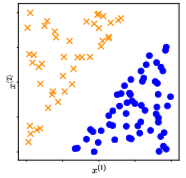
\includegraphics[width=\textwidth]{dados_linearmenteseparaveismmll}
		\caption{Dados linearmente separáveis. \label{fig4:a}}
	\end{subfigure}
	\begin{subfigure}[h]{0.31\textwidth}
		\centering
		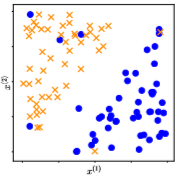
\includegraphics[width=\textwidth]{dados_nlinearmenteseparaveismml}
		\caption{Dados não linearmente separáveis. \label{fig4:b}}
	\end{subfigure}
\caption{Fonte: \textcite{Faisal2019} \label{fig4}}
\end{figure}


Neste caso, temos que o conjunto viável
\[
\{ (w,b) \in \RR^{n+1} \mid 1-y_{i}(w^{T}x^{i} + b) \leq 0 , \quad i=1, \ldots , m \}
\]
é vazio e, portanto, a formulação dada pelo problema \eqref{eq:problemageralSVM} não fornece um classificador.

Assim, no intuito de contornar esse problema utilizamos regularização para suavizar as margens, acrescentando variáveis de folga $\xi_{i} \geq 0$ associadas aos dados de treinamento $x_{i}$, com $i=1, \ldots , m$, e permitindo, assim, uma flexibilização do problema de estimar as variáveis $w$ e $b$. Em outras palavras, a restrição $1-y_{i}(w^{T}x^{i} + b) \leq 0$ é relaxada e substituída por $1-y_{i}(w^{T}x^{i} + b) \leq \xi_{i} $, com $\xi_{i} \geq 0$. Cada variável de folga $\xi_{i}$ mensura a distância que determinado dado $x_{i}$ está do seu respectivo hiperplano separador, caso este dado esteja do lado errado.

%Esta imagem também não está sendo lida, detectar problema #chateada -Uhhhul deu certo! LEMBRETE: não usar acento ao nomear figuras
\begin{figure}[!h] 
	\centering
	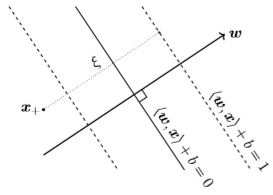
\includegraphics[width=0.40\textwidth]{mmlinterpretacao_variavel_xi}
	\caption{Variáveis de folga \label{fig5} \\ Fonte: \textcite{Faisal2019}}
\end{figure}

Tal procedimento permite que pontos da classe positiva permaneçam fora do semiespaço $\mathcal{S}^{+}=\{x\in \RR^n \mid w^{T}x+b\geq 1\}$ e/ou pontos da classe negativa fora do semiespaço $\mathcal{S}^{-}=\{x\in \RR^n \mid w^{T}x+b\leq -1\}$. 

Nesta formulação o hiperplano separador é denominado hiperplano de margem flexível e as restrições dos hiperplanos separadores são reformuladas da seguinte maneira 
\begin{align}
w^{T}x^{i}+b &\geq 1 - \xi_{i} , \text{ para  todo } x^{i} \in \Xset^{+}, \label{restricoesCSVM+} \\
w^{T}x^{i}+b &\leq -1 +\xi_{i} , \text{ para  todo } x^{i} \in \Xset^{-}. \label{restricoesCSVM-}
\end{align}


Agora nosso objetivo é encontrar $w$ e $b$ ótimos de modo a obter um bom classificador. Primeiramente, observe que dados $w$ e $b$ arbitrários, podemos escolher $\xi_{i} \geq 0$ de modo que as restrições \eqref{restricoesCSVM+} e \eqref{restricoesCSVM-} sejam satisfeitas. Para tanto, podemos definir
\[
\xi_{i} =  \left \{ \begin{array}{cc} \max\{0, 1-w^{T}x^{i}-b\}, & \quad \text{se} \quad x^{i} \in \Xset^{+}, \\
\max\{0, 1+w^{T}x^{i}+b\}, & \quad \text{se} \quad x^{i} \in \Xset^{-}.
\end{array} \right .
\]
 
Desse modo, para obter um bom classificador não basta apenas maximizar a margem definida pelos hiperplanos $\Hset^{+}$ e $\Hset^{-}$ e introduzir as variáveis de folga nas restrições, mantendo a mesma função objetivo, pois, como exemplificado por \textcite{Evelin2017}, a \Cref{fig6} ilustra o hiperplano dado por $w_{0}^{T}x+b = 0$, que não poder ser usado para classificar os dados, mas satisfaz as restrições \eqref{restricoesCSVM+} e \eqref{restricoesCSVM-}. 

\begin{figure}[!h] 
	\centering
	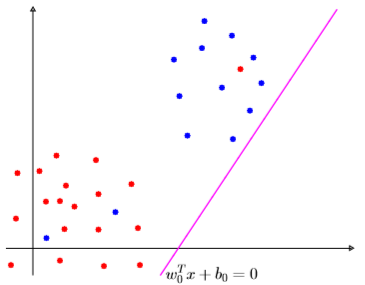
\includegraphics[width=0.40\textwidth]{restricoes_maximizacaomargem}
	\caption{Pensar. \label{fig6} \\ Fonte: \textcite{Evelin2017}}
\end{figure}
 

Portanto, para reformular o problema original de maximizar a margem é preciso também controlar o valor dessas variáveis de modo a estimular uma classificação correta, pois quanto maior o valor delas mais será permitido violar as restrições. Em vista disso, é acrescentada na função objetivo uma parcela que corresponde à penalização das violações e o problema \eqref{eq:problemageralSVM} é reformulado da seguinte forma

\[ \label{eq:problemaCSVM}
\begin{aligned}
\min_{w,b,\xi} & \quad \dfrac{1}{2} \Vert w\Vert^{2} + C \sum_{i=1}^{m} \xi_{i} \\
\text{s.a.} &  \quad y_i(w^{T}x^{i}+b) \geq 1 - \xi_{i}, \quad i=1, \ldots , m, \\
& \xi_{i} \geq 0, \quad i=1, \ldots , m,\end{aligned}
\]
%não consegui alinhar a última linha às duas primeiras
em que $C>0$ é um parâmetro de regularização que tem o objetivo de controlar a importância das variáveis de folga. O valor do parâmetro $C$ que fornece uma boa classificação dos dados é escolhido de maneira heurística na fase de treinamento, geralmente a partir da natureza do problema.É devido a utilização desse parâmetro esta modelagem de SVM também é conhecida como C-SVM.

O termo $C \sum_{i=1}^{m} \xi_{i}$ na função objetivo do problema \eqref{eq:problemaCSVM} pode ser pensado como uma medida de erro de classificação, pois minimiza o valor das variáveis de folga e reduz desse modo o número de pontos classificados incorretamente. De fato, aumentando o valor do parâmetro $C$ aumenta-se a penalização sobre a violação da restrição original do problema SVM. Por outro lado, diminuindo o valor de $C$ o modelo se torna mais flexível a esse tipo de violação. 

O problema de margem flexível \eqref{eq:problemaCSVM}, assim como o problema \eqref{eq:problemageralSVM}, também possui restrições lineares 
\begin{align} 
g_{i}(w,b,\xi) = & 1-\xi_{i} - y_i(w^{T}x^{i}+b) \leq 0 \quad \text{e} \\
h_{i}(w,b,\xi) = & - \xi_{i} \leq 0, \quad i=1, \ldots, m,
\end{align}

e assim, o conjunto viável
\[
\Omega = \{(w,b,\xi) \in \RR^{n+1+m} \mid g_{i}(w,b,\xi) \leq 0, \, h_{i}(w,b,\xi) \leq 0, \, i=1, \ldots, m \} 
\]
é um poliedro não vazio.

Ademais, a função objetivo $f$ é quadrática e limitada inferiormente em $\Omega$, pois 
\[
f(w,b,\xi) = \dfrac{1}{2} \Vert w\Vert^{2} + \underbrace{C}_{> 0} \sum_{i=1}^{m} \underbrace{\xi_{i}}_{\geq 0} \geq 0.
\]
%Assim o Teorema de Programação Quadrática (1.34) garante a existência de um minimizador global para o problema \eqref{eq:problemaCSVM}.


%-------------------------------------------------------------------------------------------------------------------------

\section{Otimização Convexa}

Em otimização uma hipótese com ótimas consequências é a convexidade, pois ela permite concluir que minimizadores locais são globais e garante que pontos estacionários são minimizadores. A partir disso, os problemas de classificação podem ser formulados em termos de otimização convexa.
Inicialmente, definimos um conjunto convexo e apresentamos alguns resultados importantes da análise convexa.

\subsection{Conjuntos Convexos}

\begin{defi} [\textcite{Ademir2013}, p. 49]
Um conjunto $C \subset \RR^{n}$ é dito convexo quando dados $x,y \in C$, o segmento $[x,y] = \{ (1-t)x + ty \mid t\in [0,1] \}$ estiver inteiramente contido em $C$.
\end{defi}

A \Cref{fig_conjuntos_convexos} apresenta a noção de convexidade de conjuntos, ilustrando um conjunto convexo e outro não convexo. Em outras palavras um conjunto convexo se caracteriza por conter todos os segmentos cujos extremos pertencem ao conjunto, o que não ocorre no segundo conjunto por exemplo.

%criar minha própria figura
\begin{figure}[!h] 
	\centering
	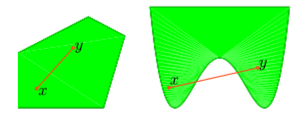
\includegraphics[width=0.40\textwidth]{conjunto_convexo}
	\caption{ Exemplo de conjunto convexo e não convexo. \label{fig_conjuntos_convexos} \\ Fonte: \textcite{Evelin2017}}
\end{figure}

Alguns exemplos de conjuntos convexos são o conjunto vazio, o espaço $\RR^{n}$, qualquer hiperplano do $\RR^{n}$ e um conjunto que contém um ponto só.

Vejamos agora alguns resultados importantes da análise convexa.

%OBS.: Apresentar a definição de norma.
\begin{lema}[\textcite{Ademir2013}, p. 50]
Considere $\Vert \cdot \Vert$ a norma euclidiana em $\RR^{n}$. Sejam $u,v \in \RR^{n}$ com $u\neq v$. Se $\Vert u \Vert = \Vert v \Vert = r$, então $\Vert (1-t)u + tv \Vert < r$, para todo $t \in (0,1)$.
\end{lema}

\begin{proof}
Seja $t \in (0,1)$ e suponha que $\Vert u \Vert = \Vert v \Vert = r$. Aplicando a desigualdade triangular, temos
\[
\Vert (1-t)u + tv \Vert \leq (1-t)\Vert u \Vert + t\Vert v \Vert = (1-t)r + tr = r.
\]

Agora, suponha por absurdo que $\Vert (1-t)u + tv \Vert = r$. Então
\[ \label{eq:lema1_convexidade_1}
(1-t)^{2} u^{T}u + 2t(1-t)u^{T}v + t^{2}v^{T}v = \Vert (1-t)u + tv \Vert = r^{2}.
\]

Como $u^{T}u = v^{T}v = r^{2}$ e $t \in (0,1)$, substituindo e desenvolvendo \eqref{eq:lema1_convexidade_1}, obtemos 
\begin{align}
r^{2} &= (1-2t+t^{2}) u^{T}u + (2t-2t^{2})u^{T}v + t^{2}v^{T}v \\
&= (1-2t+t^{2}) r^{2} + (2t-2t^{2})u^{T}v + t^{2}r^{2} \\
&= r^{2} - 2tr^{2} + t^{2}r^{2} + (2t-2t^{2})u^{T}v + t^{2}r^{2} .\\
\end{align}

Evidenciando $r^{2}$, temos
\[ 
(2t-2t^{2})r^{2} = (2t-2t^{2})u^{T}v,
\]
e, portanto,
\[ \label{eq:lema1_convexidade_2}
r^{2} = u^{T}v.
\]

Assim, por \eqref{eq:lema1_convexidade_2},
\[
\Vert u-v \Vert^{2} = u^{T}u - 2u^{T}v + v^{T}v = r^{2} - 2r^{2} + r^{2} = 0,
\]
o que é uma contradição, pois por hipótese $u \neq v$. Portanto, concluímos que $\Vert (1-t)u + tv \Vert < r$, para todo $t \in (0,1)$.
\end{proof}

Agora, dado um conjunto $S \subset \RR^{n}$ e um ponto $z \in \RR^{n}$, considere o problema de encontrar um ponto de $S$ mais próximo de $z$, em outras palavras, queremos minimizar a distânica de um ponto a um conjunto. Assim, os próximos resultados garantem a existência da solução no caso de $S$ ser um conjunto fechado e sua unicidade se, além de fechado, $S$ for convexo. Tal solução é chamada de projeção de $z$ sobre $S$, e denotada por $\proj_{S} (z)$. 

\begin{lema} [\textcite{Ademir2013}, p. 51]
Seja $S \subset \RR^{n}$ um conjunto fechado não vazio. Dado $z \in \RR^{n}$, existe $\bar{z} \in S$ tal que
\[
\Vert z - \bar{z} \Vert \leq \Vert z - x \Vert,
\]
para todo $x \in S$.
\end{lema}

\begin{lema} [\textcite{Ademir2013}, p. 52] \label{lema_existenciaprojecao_convexidade}
Seja $S \subset \RR^{n}$ um conjunto não vazio, convexo e fechado. Dado $z \in \RR^{n}$, existe um único $\bar{z} \in S$ tal que
\[
\Vert z - \bar{z} \Vert \leq \Vert z - x \Vert
\]
para todo $x \in S$.
\end{lema}

No \Cref{lema_existenciaprojecao_convexidade} denotamos $\bar{z} = \proj_{S} (z)$.

\begin{teo} [\textcite{Ademir2013}, p. 53] \label{lema_condicaoprojecao_convexidade}
Sejam $S \subset \RR^{n}$ um conjunto não vazio, convexo e fechado, $z \in \RR^{n}$ e $\bar{z} = \proj_{S} (z)$. Então, 
\[
(z - \bar{z})^{T}(x - \bar{z}) \leq 0 ,
\]
para todo $x \in S$.
\end{teo}

O \Cref{lema_condicaoprojecao_convexidade} estabelece uma condição necessária e suficiente para caracterizar a projeção. Este resultado é provado no lema seguinte.

\begin{lema} [\textcite{Ademir2013}, p. 54] \label{lema_defineprojecao_convexidade}
Sejam $S \subset \RR^{n}$ um conjunto não vazio, convexo e fechado e $z \in \RR^{n}$. Se $\bar{z} \in S$ satisfaz
\[
(z - \bar{z})^{T}(x - \bar{z}) \leq 0 ,
\]
para todo $x \in S$, então $\bar{z} = \proj_{S} (z)$.
\end{lema}

O \Cref{lema_defineprojecao_convexidade} fornece uma condição necessária de otimalidade ao minimizar uma função em um conjunto convexo fechado.

\begin{lema} [\textcite{Ademir2013}, p. 54]
Sejam $f: \RR^{n} \rightarrow \RR$ uma função diferenciável e $C \subset \RR^{n}$ convexo e fechado. Se $x^{*} \in C$ é minimizador local de $f$ em $C$, então
\[
\proj_{C} (x^{*} - \alpha \nabla f(x^{*})) = x^{*} ,
\]
para todo $\alpha \geq 0$.
\end{lema}

\subsection{Funções Convexas}

\begin{defi} [\textcite{Ademir2013}, p. 56] \label{defi:funcao_convexa}
Seja $C \subset \RR^{n}$ um conjunto convexo. Dizemos que a função $f: \RR^{n} \rightarrow \RR$ é convexa em $C$ quando
\[
f((1-t)x + ty) \leq (1-t)f(x) + tf(y),
\]
para todos $x,y \in C$ e $t \in [0,1]$.
\end{defi}

A noção geométrica da \Cref{defi:funcao_convexa} é apresentada na \Cref{fig_funcao_convexa}, em que qualquer arco do gráfico de uma função convexa está sempre abaixo do segmento que liga as extremidades.

%criar minha própria imagem
\begin{figure}[!h] 
	\centering
	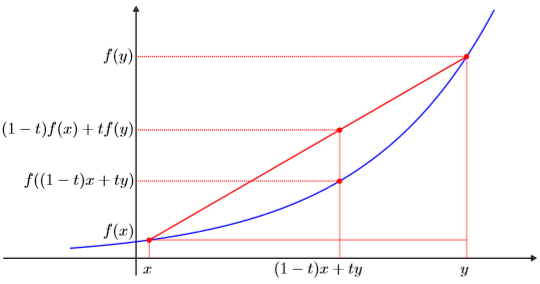
\includegraphics[width=0.85\textwidth]{funcao_convexa}
	\caption{ Função Convexa. \label{fig_funcao_convexa} \\ Fonte: \textcite{Evelin2017}}
\end{figure}

\begin{obs}
Todo problema de maximização
\[
\begin{aligned}
\max_{x} & \quad f(x) \\
\text{s.a.} & \quad x \in \Omega \end{aligned}
 \]
pode ser transformado em um problema de minimização equivalente
\[
\begin{aligned}
\min_{x} & \quad -f(x) \\
\text{s.a.} & \quad x \in \Omega .\end{aligned}
 \]
\end{obs}

\begin{defi} [\textcite{Izmailov2014ac}, p. 80]
Se $D \subset \RR^{n}$ é um conjunto convexo, dizemos que $f: D \rightarrow \RR $ é uma \emph{função côncava} em $D$, quando a função $(-f)$ é convexa em $D$.
\end{defi}

Assim, maximizar uma função côncava num conjunto convexo equivale a minimizar uma função convexa num conjunto convexo.

O teorema seguinte justifica o fato da convexidade ser uma propriedade tão importante em otimização.

\begin{teo} [\textcite{Ademir2013}, p. 57]
Sejam $C \subset \RR^{n}$ um conjunto convexo e $f:C \rightarrow \RR$ uma função convexa. Se $x^{*} \in C$ é minimizador local de $f$, então $x^{*}$ é minimizador global de $f$.
\end{teo}
\begin{proof}
Seja $x^{*}$ um minimizador local de $f$. Então, existe $\delta > 0$ tal que $f(x^{*}) \leq f(x)$, para todo $x \in B(x^{*}, \delta) \cap C$. Dado $y \in C$, tal que $y \notin B(x^{*}, \delta)$, e tome $t \in (0,1]$ de modo que $t \Vert y-x^{*} \Vert < \delta$. Assim, o ponto $x = (1-t)x^{*} + ty$ satisfaz
\[
\Vert x - x^{*} \Vert = \Vert (1-t)x^{*} + ty - x^{*} \Vert = \Vert x^{*} - tx^{*} + ty - x^{*} \Vert = t \Vert y - x^{*} \Vert < \delta ,
\]
e, portanto, $x \in B(x^{*}, \delta) \cap C$.

Desse modo, como $C$ é um conjunto convexo, temos
\[
f(x^{*}) \leq f(x) \leq (1-t)f(x^{*}) + tf(y) = f(x^{*}) + t(f(y)-f(x^{*})),
\]
donde segue que $f(x^{*}) \leq f(y)$.

Portanto, $x^{*}$ é minimizador global de $f$.
\end{proof}

A seguir apresentamos outra forma de caracterizar a convexidade de uma função quando temos hipóteses de diferenciabilidade.

\begin{teo} [\textcite{Ademir2013}, p. 58]
Sejam $f: \RR^{n} \rightarrow \RR $ uma função diferenciável e $C \in \RR^{n}$ um conjunto convexo. A função $f$ é convexa em $C$ se, e somente se, 
\[
f(y) \geq f(x) + \nabla f(x)^{T}(y-x),
\]
para todos $x, y \in C$.
\end{teo}

\begin{proof}
Seja $f$ uma função convexa. Para $x,y \in C$ e $t \in (0,1]$ quaisquer, temos $(1-t)x + ty = x + t(y-x)$, pois $C$ é convexo. Assim, definindo $d = y-x$, temos que $x + td \in C$ e
\[
f(x+td) = f((1-t)x + ty) \leq (1-t)f(x) + tf(y),
\]
logo
\[
f(x+td) \leq f(x) + t(f(y)-f(x)),
\]
o que implica em 
\[
f(y)-f(x) \geq \dfrac{f(x+td)-f(x)}{t} .
\]

Passando o limite quando $t \rightarrow 0^{+}$, temos
\[
f(y)-f(x) \geq \lim_{t \rightarrow 0^{+}} \dfrac{f(x+td)-f(x)}{t} = \nabla f(x)^{T} d = \nabla f(x)^{T} (y-x) ,
\]
e, portanto,
\[
f(y) \geq f(x) + \nabla f(x)^{T} (y-x) .
\]

Reciprocamente, considere $z = (1-t)x + ty$ e observe que 
\[
f(x) \geq f(z) + \nabla f(z)^{T}(x-z) \quad \text{e} \quad f(y) \geq f(z) + \nabla f(z)^{T}(y-z) .
\]

Agora, multiplicando a primeira desigualdade por $(1-t)$ e a segunda por $t$, obtemos
\begin{align}
(1-t)f(x) + tf(y) & \geq (1-t)(f(z) + \nabla f(z)^{T}(x-z)) + t(f(z) + \nabla f(z)^{T}(y-z)) \\
& \geq f(z) - tf(z) -t\nabla f(z)^{T}(x-z) + tf(z) + t\nabla f(z)^{T}(y-z) \\ %dúvida nessa passagem - rever demonstração
& \geq f((1-t)x + ty) .
\end{align}

Portanto, a função $f$ é convexa em $C$.
\end{proof}


\newpage

\printbibliography
\end{document}